\documentclass[conference]{IEEEtran}
\IEEEoverridecommandlockouts

\usepackage{cite}
\usepackage{amsmath,amssymb,amsfonts}
\usepackage{algorithmic}
\usepackage{xcolor}
\usepackage{textcomp}
\usepackage[dvipdfmx]{graphicx,hyperref}
\usepackage[subrefformat=parens]{subcaption}

\captionsetup[subfigure]{labelformat=simple}
\renewcommand{\thesubfigure}{(\alph{subfigure})}

\hypersetup{
    setpagesize=false,
	bookmarksnumbered=true,
	bookmarksopen=true,
	colorlinks=true,
	linkcolor=black,
	citecolor=black,
    urlcolor=black,
}

\def\BibTeX{
    {\rm B\kern-.05em{\sc i\kern-.025em b}\kern-.08em T\kern-.1667em\lower.7ex\hbox{E}\kern-.125emX}
}


\begin{document}

    \title{
        Liver Tumor Detection and Classification from Abdominal Ultrasound Images with CenterNet Using Contrastive Learning
    }

    \author{
        \IEEEauthorblockN{
            Eigo Hara$^\dagger$, Keisuke Doman$^\dagger$, Yoshito Mekada$^\dagger$, Naoshi Nishida$^\ddagger$, and Masatoshi Kudo$^\ddagger$
        }
        \IEEEauthorblockA{
            $\dagger$ School of Engineering, Chukyo University, Japan\\
            $\ddagger$ Faculty of Medicine, Kindai University, Japan\\
            Email: hara.e@md.sist.chukyo-u.ac.jp, \{kdoman, y-mekada\}@sist.chukyo-u.ac.jp, \{naoshi, m-kudo\}@med.kindai.ac.jp
        }
    }

    \maketitle

    \begin{abstract}
        We propose a method for simultaneously detecting and classifying liver tumors from abdominal ultrasound images.
        The proposed method uses CenterNet as a detection model, and also uses SimSiam-based contrastive learning to obtain effective features for both.
        The proposed method could achieve a high accuracy comparable to our previous method.
    \end{abstract}

    \begin{IEEEkeywords}
        tumor detection and classification, contrastive learning, ultrasonography
    \end{IEEEkeywords}

    \section{Introduction}
        Abdominal ultrasonography is a difficult task, and computer-assisted diagnosis, e.g. detection and classification of abdominal tumors, is required.
        We previously studied a two-stage method for detection\cite{prestudy_det} and classification\cite{prestudy_cls} of abdominal tumors, and its detection and classification accuracies were both about 90\%.
        The method first detects tumors and then classifies their types by using independent two deep learning models.
        This paper proposes a one-stage method using contrastive learning for simultaneous detection and classification.
        This approach can learn effective features for both tasks, which leads to mutually improving each performance.

        \section{Proposed Method}
        The proposed method uses CenterNet\cite{centernet} for liver tumor detection and classification from abdominal ultrasound images as shown in Fig.\ref{fig:architecture}, considering a circular shape of a liver tumor.
        The backbone in CenterNet is first trained through contrastive learning with SimSiam\cite{simsiam} (Fig.~\ref{fig:simsiam}), and then fine-tuned (Fig.~\ref{fig:centernet}).
        SimSiam has a simple structure and can learn effective features for both tasks even with small batch sizes.
        By this framework, the method outputs the positions and sizes, and the types (heatmaps) of liver tumors from input images.

    \section{Experiments}
        We investigated the effectiveness of the proposed method through experiments by comparing it with our previous method\cite{prestudy_det,prestudy_cls}, which separately uses YOLOv3 and VGG16 as detection and classification models.
        We used 83,903 abdominal ultrasound images and divided them into 8:1:1 for training, validation, and test sets.

        Experimental results are shown in Table~\ref{tab:metric_center_stepwise}.
        The proposed method, a one-stage method with CenterNet, could achieve a high accuracy comparable with the previous method, which is a two-stage method.
        From the result, we confirmed the effectiveness of the proposed method.

        \begin{figure}[t]
            \centering
            \begin{minipage}[t]{.36\linewidth}
                \centering
                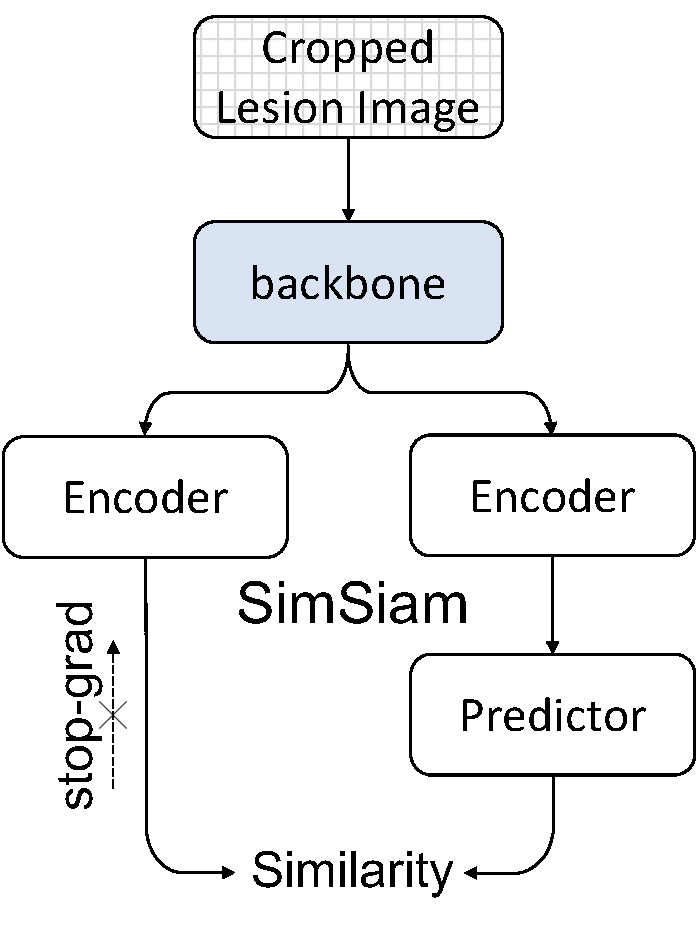
\includegraphics[width=\linewidth]{../../fig/simsiam_s.pdf}
                \subcaption{Contrastive learning}
                \label{fig:simsiam}
            \end{minipage}
            \begin{minipage}[t]{.6\linewidth}
                \centering
                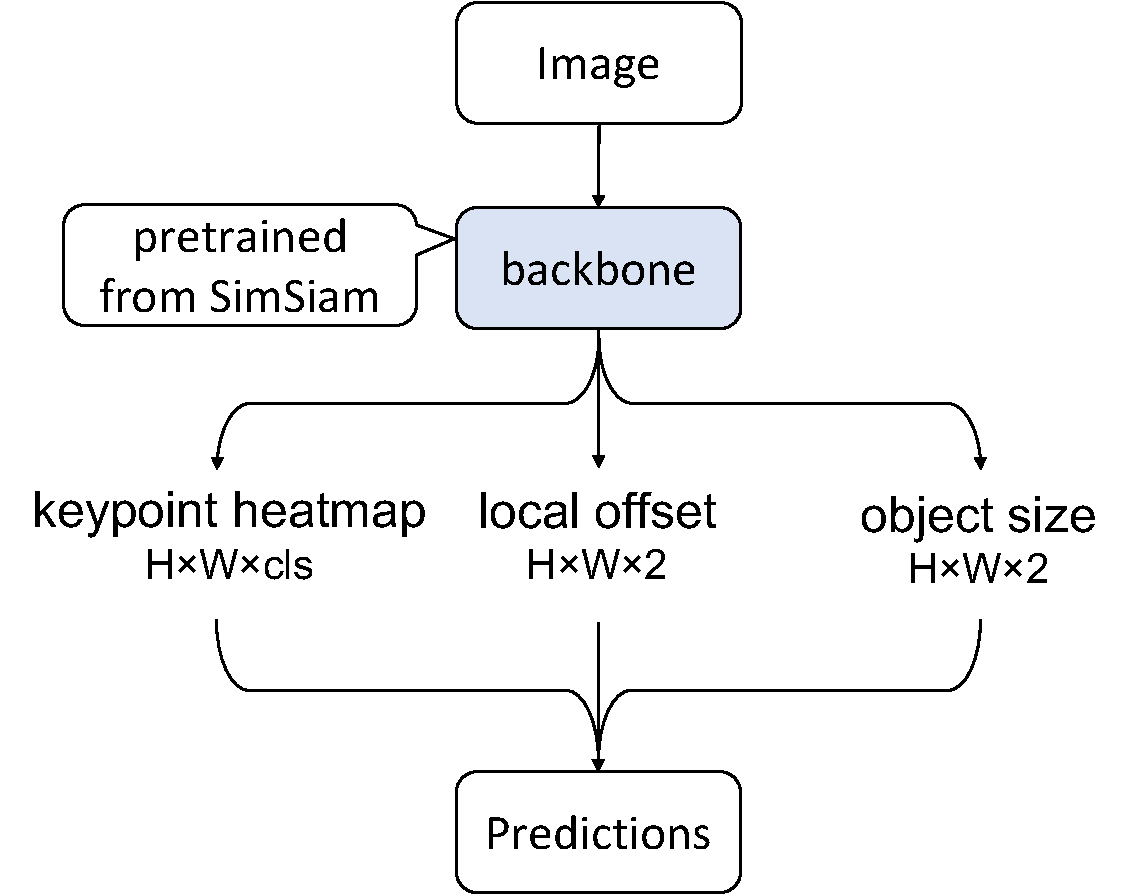
\includegraphics[width=\linewidth]{../..//fig/centernet_s.pdf}
                \subcaption{CenterNet-based model}
                \label{fig:centernet}
            \end{minipage}
            \caption{Architecture of the proposed method}
            \label{fig:architecture}
        \end{figure}

        \begin{table}[t]
            \centering
            \caption{Experimental results: Accuracy comparison}
            \label{tab:metric_center_stepwise}
            \begin{tabular}{l|cc|c} \hline
                \multicolumn{1}{c|}{Method} & F1$_{det}$ & Acc$_{cls}$ & Correct Rate \\ \hline
                Previous\cite{prestudy_det,prestudy_cls} & 0.8750 & 0.8909 & 0.7795 $(\approx 0.8750 \times 0.8909)$ \\
                Proposed & 0.8456 & 0.9206 & 0.7785 $(\approx 0.8456 \times 0.9206)$ \\ \hline
            \end{tabular}
        \end{table}

    \section{Conclusion}
        We proposed a one-stage method for simultaneous detection and classification of liver tumors from abdominal ultrasound images with CenterNet using SimSiam-based contrastive learning.
        We confirmed that the proposed method could achieve a high classification accuracy comparable with our previous two-stage method.
        We will study the improvement of CenterNet, e.g., by separating the classification head from the keypoint heatmap one from the backbone.

    \begin{thebibliography}{9}
        \bibitem{prestudy_det} S. Yamagishi et al.: ``Detection and tracking of liver tumors for ultrasound diagnostic support using deep learning,'' J. Image and Graphics, 10(1):50--55, 2021.
        \bibitem{prestudy_cls} N. Nishida et al.: ``Artificial intelligence (AI) models for the ultrasonographic diagnosis of liver tumors and comparison of diagnostic accuracies between AI and human experts,'' J. Gastroenterol, 57(4):309--321, 2022.
        \bibitem{centernet} X. Zhou et al.: ``Objects as Points,'' arXiv preprint, arXiv:1904.07850, 2019.
        \bibitem{simsiam} X. Chen and K. He: ``Exploring simple siamese representation learning,'' Proc. 2021 IEEE/CVF Conf. on Computer Vision and Pattern Recognition, 15750--15758, 2021.
    \end{thebibliography}

\end{document}
